\section{Component View}
The purpose of this section is to show the component diagram which is intended to represent the internal structure of the modeled software system in terms of its main components and the relationships among them.

The following legend is used:
\begin{center}
    \begin{figure}[h!]
  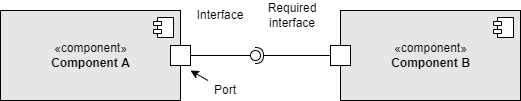
\includegraphics[width=\textwidth,height=\textheight,keepaspectratio]{./Images/Component legend.png}
  \caption{Component legend}
\end{figure}
\end{center}

All components within the diagram are described in detail below.
\begin{itemize}

\item \textbf{WebApplication}: it manages all user interactions with the web application and associates them with the required functions.
It deals with managing all notifications addressed to a specific user.

\item \textbf{MobileApplication}: it manages all user interactions with the mobile application and associates them with the required functions.
It deals with managing all notifications addressed to a specific user.

\item \textbf{AuthenticationService}: it is a service that is involved when login is performed (both from the mobile app and the web app). It checks user permissions according to the role she/he has.
In order to verify the credentials inserted by the user, this component is directly connected with DatabaseAccess component. 

\item \textbf{RegistrationService}: it manages the registration of a unregistered user; in particular, it allows to retrieve farmer's position thanks to the connection to GoogleMapsAPI component. It also accesses the database managed by the Telangana government to check the validity of the ID code entered by the policy maker and agronomist during registration in DREAM. Access to this database takes place thanks to the TelanganaGovernmentService component.
In order to store the new user in the database, the component must be connected to the DatabaseAccess component. 
RegistrationService component includes the following subcomponent.

\begin{itemize}

\item \textbf{EmailManager}: it is necessary when a user who has not yet registered wants to register. To verify his/her email during registration, the system automatically sends a confirmation email to the user and activates a 10-minute timer within which the user must confirm his/her registration.
\end{itemize}
\item \textbf{PolicyMakerService}: This component includes the following subcomponents.

\begin{itemize}
    \item \textbf{TimeChartService}: it computes and displays Telangana’s farmers data in a graph so that the policy maker can analyze the various parameters of interest over time.  In order to collect all the data of interest, the component must be connected to the DatabaseAccess component. 
    \item \textbf{MapService}: it computes and displays Telangana’s farmers performance map using some filters. In order to collect all the data of interest, the component must be connected to the DatabaseAccess component. The connection to GoogleMapsAPI component allows to process the map to be displayed. 
\end{itemize}

\item \textbf{AgronomistService}: This component includes the following subcomponents.

\begin{itemize}
    \item \textbf{HelpResponseService}: it allows an agronomist to manage the response to a help request received. In order to retrieve all the help requests with a certain agronomist as a recipient and store the new help response created by him/her, the component must be connected to the DatabaseAccess component. 
    \item \textbf{MandalMapService}: it retrieves and displays relevant personal data of farmers and their performance score on the map of a mandal. This component is closely linked to the TableService component, which is called up as soon as the agronomist selects a farmer of interest on the map. Obviously, in order to collect all the data of interest, the component must be connected to the DatabaseAccess component. 
    The connection to GoogleMapsAPI component allows to process the map to be displayed.
    \item \textbf{TableService}: it retrieves and displays the table of farmers’ performance in descending order based on their performance score. Obviously, in order to collect all the data of interest, the component must be connected to the DatabaseAccess component.
    \item \textbf{DailyPlanService}: it deals with the creation and updating and confirmation of the daily plan of a agronomist. Specifically, it guarantees that for each farmer there are at least two visits per year by the responsible agronomist. To retrieve the scheduled plan, this component must be connected with DatabaseAccess component.
    \item \textbf{WeatherForecastsService}: it collects the data related to the weather forecasts in the mandal of a certain agronomist according to the date selected by the agronomist. To retrieve weather forecasts, it needs to be connected to the external API TelanganaGovernmentService component. 
    The connection to CopernicusClimateDataStoreService component allows to retrieve soil moisture in the mandal.
    These data are placed on the appropriate mandal map thanks to an external API component: GoogleMapsAPI.
\end{itemize}

\item \textbf{FarmerService}: This component includes the following subcomponents.

\begin{itemize}
    \item \textbf{HelpRequestService}: it is necessary for the creation and subsequent management of help requests by the farmer. The connection to DatabaseAccess component allows it to retrieve the recipients to whom the request can be sent (agronomist in charge of the mandal and well performing farmers).\\
    In addition, if a (well performing) farmer has received a help request from another farmer, this component takes care of managing the function that allows the farmer to respond to the request.
    \item \textbf{DiscussionForumService}: it manages the creation of threads by a farmer on the discussion forum, the creation of posts in response to a specific thread (always by other farmers) and the search by topic of a thread already created. It also performs these functions thanks to the connection to the DatabaseAccess component.
    \item \textbf{VisitService}: it retrieves the visits scheduled for a farmer that corresponds to the daily plan of an agronomist.
    Since visits are stored in the database, to retrieve them, this component must be connected to the DatabaseAccess component.
    \item \textbf{PerformanceService}: it takes care of updating a farmer's performance data every time he/she enters new data about his/her crop. It is connected to the DatabaseAccess component not only to store the computed performance but also to get farmer's position and his/her last performance date (to take into account the right time interval for which performance has to be computed).
    It also is connected to external API TelanganaWaterIrrigationService to compute the quantity of water consumed. Furthermore it is linked to WeatherConditionService component which allows to retrieve weather conditions and soil moisture.
    \item \textbf{WeatherConditionService}: it collects the data related to weather conditions based on the farmer's position. To accomplish this task, it needs to be connected to the external API TelanganaGovernmentService as well as to the CopernicusClimateDataStoreService component. It also has to be connected to DatabaseAccess component to retrieve farmer's position.
    \item \textbf{SuggestionsService}: it is used to elaborate farmer's suggestions based on his/her relevant information regarding his/her production and the position of his/her farm. These data are obtained thanks to the connection to the DatabaseAccess and WeatherConditionService components.
\end{itemize}

\item \textbf{DatabaseAccess}: it is responsible to retrieve (and store) data from (to) a data source. In this case, it manages the access to the database.

\item \textbf{Database}: This component includes the following subcomponent.

\begin{itemize}
    \item \textbf{DBMS}: Database Management System refers to a software that allow users to access databases and manipulate, maintain, report, and relate data. It is used to reduce data redundancy, share data in a controlled manner, and reduce data integrity issues.
\end{itemize}

\item \textbf{ExternalAPIs}: This component includes the following subcomponents.

\begin{itemize}
    \item \textbf{GoogleMapsAPI}: it allows the connection of the application to Google Maps APIs. All functions that require access to geographical data, not yet saved in the internal database, will rely on this component.
    \item \textbf{CopernicusClimateDataStoreService}: it is responsible for retrieving soil moisture data in the Telangana region.
    \item \textbf{TelanganaGovernmentService}: it takes care of retrieving data relating to weather conditions in Telangana region. It also used to access ID codes' DB managed by Telangana government to check validity of ID code inserted by policy makers and agronomist while registering into DREAM. 
    \item \textbf{TelanganaWaterIrrigationService}: it is responsible for retrieving the amount of water consumed by each farmer in the Telangana region.
\end{itemize}

\end{itemize}


\def\fillandplacepagenumber{%
 \par\pagestyle{empty}%
\vbox to 0pt{\vss}\vfill
\vbox to 0pt{\baselineskip0pt
   \hbox to\linewidth{\hss}%
   \setlength{\footskip}{70pt}
   \baselineskip\footskip
   \hbox to\linewidth{%
     \hfil\thepage\hfil}\vss}}

\begin{landscape}
\begin{figure}[h]
\vspace*{-2cm}
\noindent
\centering
\centerline{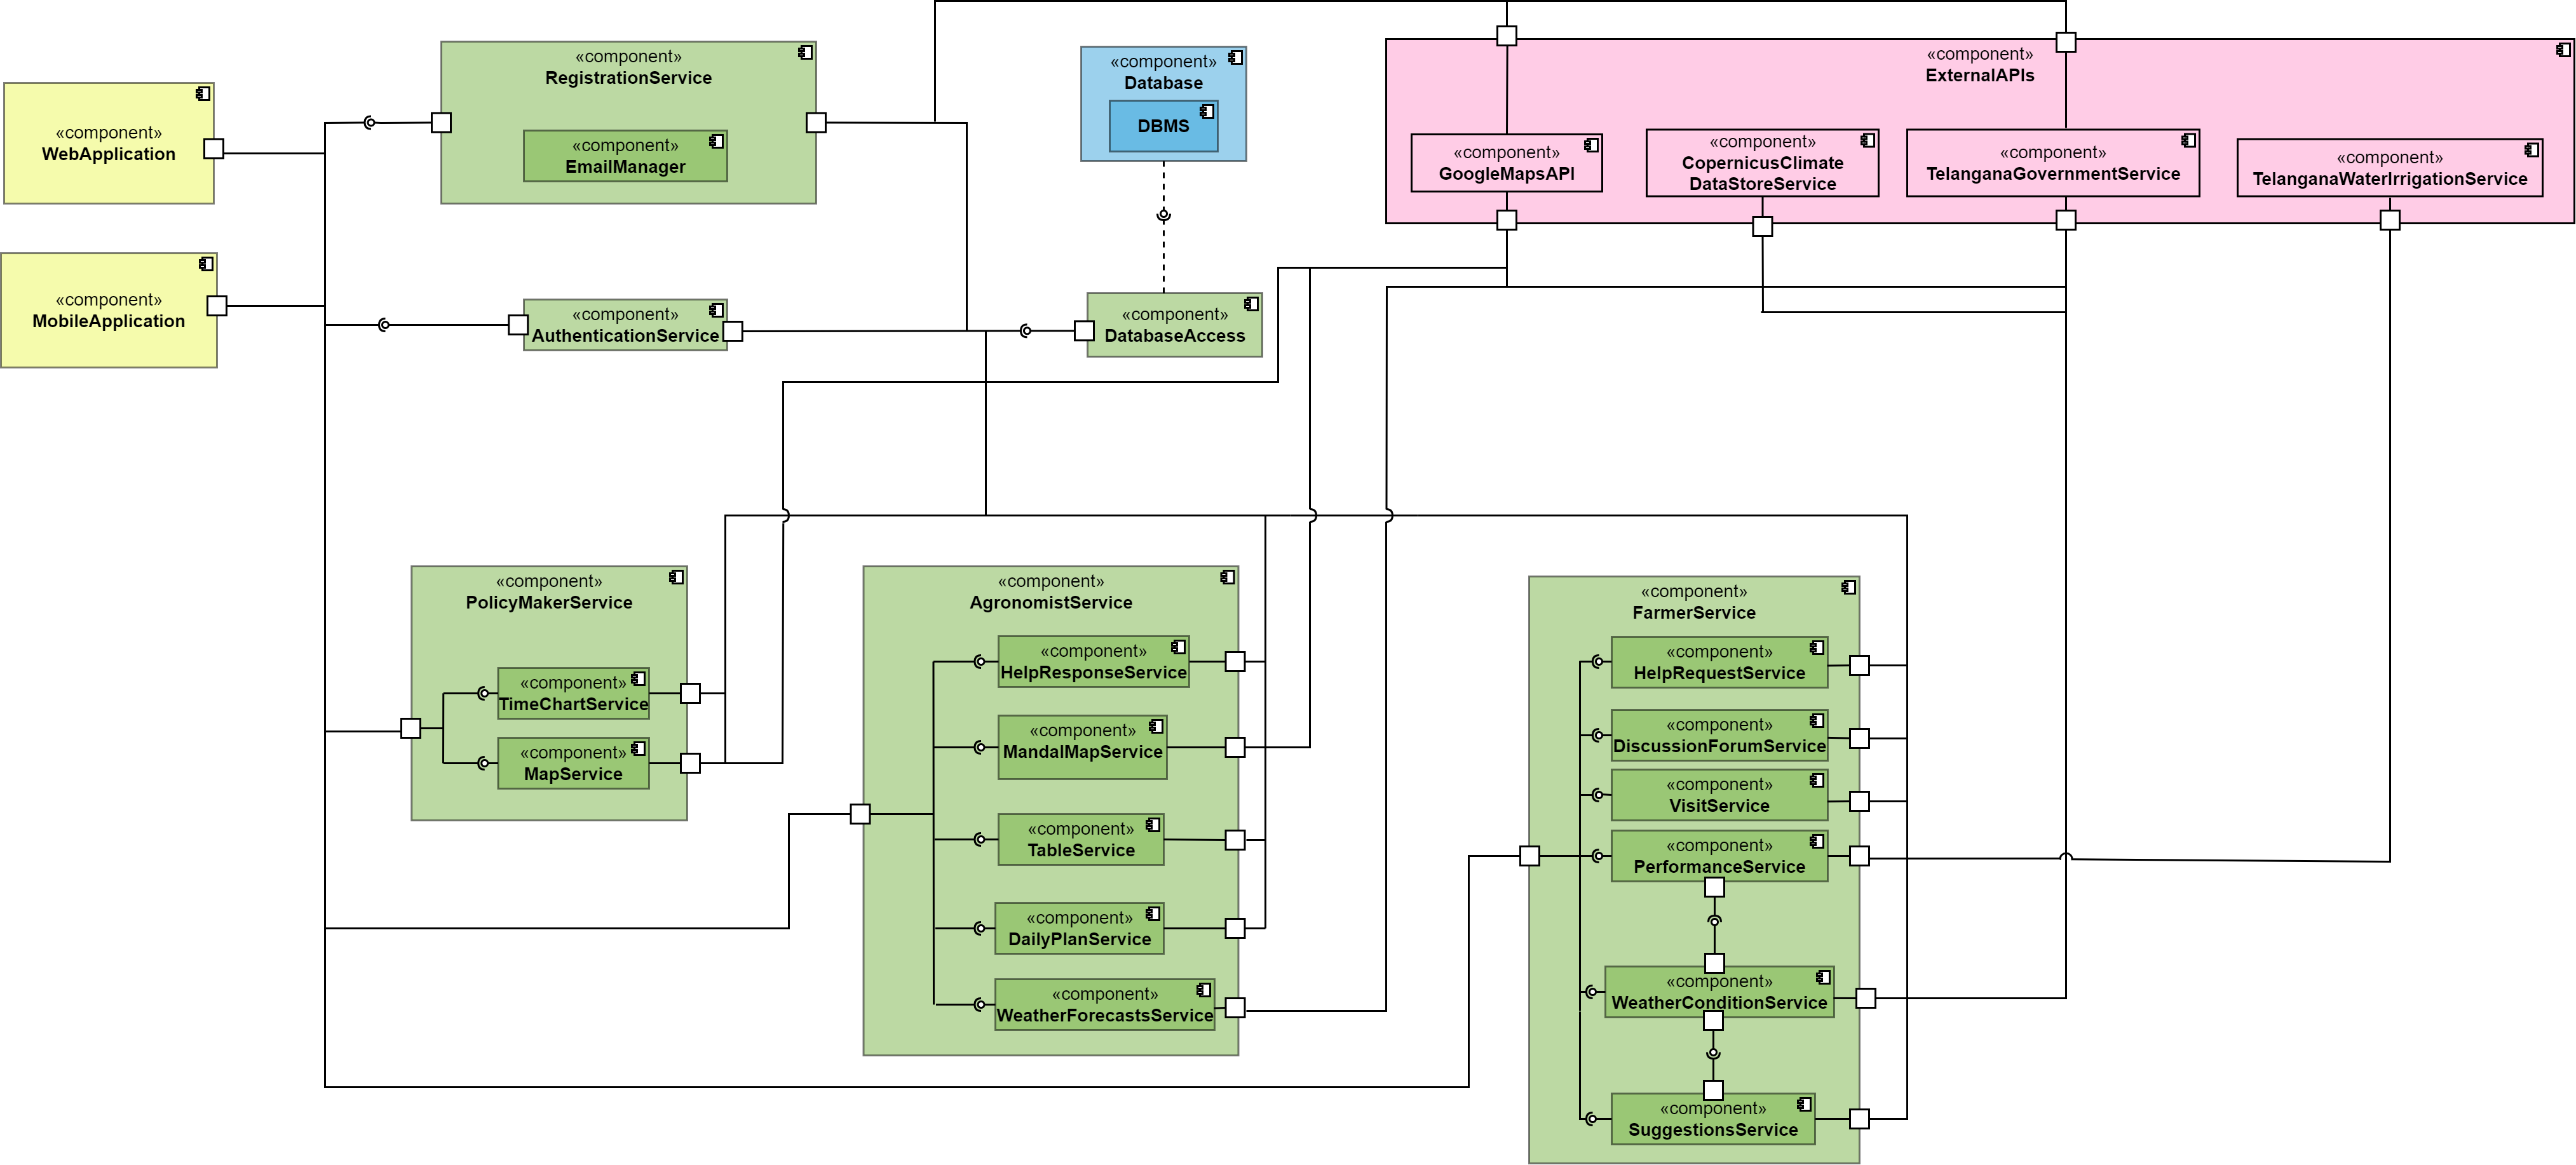
\includegraphics[scale = 0.2]{./Images/Component diagram.png}}
    \caption{Component diagram}
    \vspace*{-12cm}
\end{figure}
\fillandplacepagenumber
\end{landscape}

